% File project.tex
%% Style files for ACL 2021
\documentclass[11pt,a4paper]{article}
\usepackage[hyperref]{acl2021}
\usepackage{times}
\usepackage{booktabs}
\usepackage{todonotes}
\usepackage{latexsym}
\usepackage{float}
\usepackage{caption}
\usepackage{subcaption}
\usepackage{enumitem}
\usepackage[normalem]{ulem}
\renewcommand{\UrlFont}{\ttfamily\small}
% This is not strictly necessary, and may be commented out,
% but it will improve the layout of the manuscript,
% and will typically save some space.
\usepackage{etoolbox} 
\AtBeginEnvironment{itemize}{\setlength\parskip{0pt}}
\AfterEndEnvironment{itemize}{\vspace*{-\dimexpr\parskip\relax}}
\usepackage{microtype}

% \titlespacing*{\section}
% {0pt}{0pt}{0pt}
% \titlespacing*{\subsection}
% {0pt}{0pt}{0pt}
% \titlespacing*{\subsubsection}
% {0pt}{0pt}{0pt}



\aclfinalcopy 

\newcommand\BibTeX{B\textsc{ib}\TeX}

\title{11-777 Spring 2021 Class Project}

\author{
  Andrew Singh\thanks{\hspace{4pt}Everyone Contributed Equally -- Alphabetical order} \hspace{2em} Ankit Ramchandani$^*$ \hspace{2em} Vashisth Parekh$^*$ \\
  \texttt{\{andrewsi, aramchan, vparekh\}@andrew.cmu.edu}
  }

\date{}

\begin{document}
\maketitle
\begin{abstract}
Template for 11-777 Reports using the ACL 2021 Style File 
\end{abstract}

\section{Introduction and Problem Definition (1-1.25 pages)}
\textbf{Thesis statement or Hypothesis we are aiming to prove}\\
``Our approach is better is not a hypothesis"

\clearpage
\section{Related Work and Background}
\label{sec:rel-work}
\subsection{ALFRED}
\label{ssec:alf}
Though ALFRED is a relatively new task, a multitude of approaches have recently been proposed that demonstrate improved performance over the baseline introduced in \cite{shridhar2020alfred}. The baseline model consists of a CNN to encode the visual input at each timestep, a bi-LSTM to encode the language directives, and a decoder LSTM to infer the action at each timestep while attending over the language encoding. \cite{corona2020modularity} used the same architecture as the baseline, except they maintained separate modules for each \emph{subgoal type} (e.g., GOTO, PICKUP). They then used a high-level controller to choose which module to execute at each step based on the language directives. \cite{singh2020moca} proposed a vision module for generating interaction masks and an action module for predicting actions, with the vision module first predicting the class of the object of interest and then generating the pixel-wise interaction mask given the predicted object class. \cite{Storks2021AreWT} addressed ALFRED's long action sequences by training the model to execute one subgoal at a time rather than all subgoals at once, and they address the agent's poor navigation performance by augmenting the agent's perception with additional viewing angles that are used for training an object detection module and for predicting the agent's orientation angle relative to the goal.

Unlike methods that learn a direct mapping from observations to actions end-to-end, \cite{Saha2021AMV} proposed a truly modular framework that is able to learn from unaligned or weakly aligned data as opposed to requiring expert demonstrations. Their mapping module includes a novel mapping scheme based on graph convolutional networks \cite{kipf2016semi} for improved navigation, and their language module leverages a pre-trained model to perform joint intent detection and slot filling on the language directives.

While the previously mentioned works improve upon the modeling approach proposed in the original ALFRED paper, \cite{Shridhar2020ALFWorldAT} also proposed a new environment to address the challenge of generalizing to unseen tasks. They aligned tasks in ALFRED with a purely textual environment, TextWorld \cite{Ct2018TextWorldAL}, allowing agents to first learn in an abstract setting in order to generalize better in the embodied setting. They additionally introduced a modular architecture to demonstrate the effectiveness of their ALFWorld environment, consisting of a state estimator that translates visual observations to text, an abstract text agent pre-trained in TextWorld that generates high-level actions from textual observations and a goal, and a controller that translates high-level actions to sequences of low-level actions in the embodied environment.

To the best of our knowledge, the papers discussed above cover all of the approaches proposed thus far that attempt the full ALFRED task.

\subsection{Related Tasks}
\subsubsection{Vision and Language Navigation}
\label{ssec:vln}
While ALFRED requires navigation and interaction with objects based on visual and language input, a related task is just vision and language based navigation (VLN). \cite{fried2018speaker} proposed a policy consisting of two modules: an instruction follower model that produced a step-by-step action sequence from visual and textual input, and a speaker model that predicted the probability that a particular language instruction describes a given sequence. To predict the final trajectory, multiple trajectories were first generated by the follower model, and the one most likely to match with the natural language description (as assessed by speaker model) was chosen. \cite{wang2019reinforced} proposed an improvement over the previous method by learning a LSTM \cite{hochreiter1997long} and attention-based policy using reinforcement learning (RL). They also used a ``speaker model'' which was used to generate an intrinsic reward for the RL algorithm based on the probability of the language description matching the predicted action sequence. \cite{wang2018look} proposed a method to jointly perform imitation and reinforcement learning using a policy that consisted of an ``action predictor'' used to predict the final action based on inputs coming from model-free and model-based RL modules. The model-free module was an LSTM and attention-based network similar to other approaches \cite{shridhar2020alfred, wang2019reinforced}. The model-based module ``imagined'' multiple different trajectories in the future, and produced a combined representation to the action predictor. \cite{wani2020multion} performed several experiments on a long-horizon navigation task in a realistic 3D setting to empirically show that using a semantic map-like memory can significantly boost navigation performance. \cite{hao2020learning} pre-trained their model on image-text-action triplets in a self-supervised manner. Their model was able to generalize better in unseen environments, improving the SOTA in the Room-to-Room task (similar to ALFRED). \cite{majumdar2020improving} improved VLN performance by using a visiolinguistic transformer based model that scores the compatibility between an instruction and a particular visual scene. Pretraining on the image-text pairs from the web improved the performance of the VLN.

\subsubsection{Embodied Question Answering}
\label{ssec:eqa}
Embodied Question Answering \cite{Das2018EmbodiedQA} (EmbodiedQA) is a related task in which an agent spawns at a random location in a 3D environment and is asked a question about an object. To correctly answer, the agent must navigate the environment and gather information through egocentric vision about the object and its surroundings. This challenging task requires many of the skills needed in the ALFRED benchmark, including active perception, commonsense reasoning, goal-driven navigation, and grounding language to vision and actions. 

\cite{Das2018EmbodiedQA} proposed an approach with a two-step navigation module: a planner that selects actions and a controller that executes those actions a variable number of times. Their agent is initialized via imitation learning and then fine-tuned via reinforcement learning. \cite{Das2018NeuralMC} improved upon this approach by introducing a high-level policy that proposes compositional sub-goals to be executed by sub-policies. They train their model via imitation learning in a bottom-up fashion, first training the sub-policies before training the high-level policy. They then fine-tune their model via reinforcement learning in a similar bottom-up fashion, allowing the high-level policy to adapt to the behavior of the sub-policies.

\cite{Yu2019MultiTargetEQ} generalized the EmbodiedQA task to multiple targets; instead of a question asking only about a single object, it may ask about several objects and require comparative reasoning. They propose a novel architecture for the task consisting of four modules: a program generator that converts the question to executable sub-programs, a navigator that executes these sub-programs to guide the agent to relevant locations, a controller that selects relevant observations along the agent's path, and a visual question answering module that uses the observations from the controller to predict the final answer.

\subsection{Relevant ML Methods}
\subsubsection{Multimodal Alignment}
\label{ssec:mmml}
In ALFRED, the agent receives all natural language instructions at the beginning of the episode, but receives visual observations at each time-step. It is imperative for the agent to align the natural language directives with its current visual observation so that it can spot objects of interest described in natural language in the current visual scene. In this section, we summarize some research in multimodal machine learning focused on this problem of learning such soft alignment \cite{baltruvsaitis2018multimodal}.

\cite{Chen2004Grounding} used a graphical model to align objects in (egocentric) images with spoken words. \cite{mei2015listen} uses a bi-LSTM with a multi-level aligner to map instructions with navigational actions. \cite{ma2019selfmonitoring} proposed a visual textual co-grounding alignment mechanism and a corresponding progress monitor. They used the hidden state from the previous timestep of their LSTM to generate textual and visual grounding, which helps their agent decide which action to take next. Similarly, \cite{wang2019reinforced} used an LSTM to predict actions and included an attention mechanism on visual and textual input based on the current hidden state of the LSTM. \cite{ke2019tactical} used attention mechanism over language to compute how the previous action aligned with the description. \cite{wang2018look, shridhar2020alfred} both used modules which  perform attention over textual input using the hidden state of the LSTM, so that the agent knows which words in the input text to focus on.

\subsubsection{Generalization in Multimodal Settings}

The ALFRED dataset has unseen splits of validation and test data which measure generalization of the learned policy, but multimodal models are more prone to overfitting due to their increased capacity \cite{wang2020makes}. To this end, \cite{wang2020makes} also proposed a gradient blending approach, which computes optimal blends of modalities based on overfitting behavior. This approach achieves SOTA results on egocentric action task similar to ALFRED. \cite{alet2019modular} presented a meta-learning strategy where they separately trained each modular component on related tasks and then combined them to create a more general model that scales across tasks. More specifically to ALFRED, \cite{nguyen2018multitask} proposed multi-task learning approach that enables visual-language representations that can be generalized to other tasks. Their algorithm used representation encoders that learn hierarchical features by fusing visual and semantic representations and task specific decoders that decode those features however they see best fit for the given task.

\subsubsection{Reinforcement and Imitation Learning}
\label{ssec:rlil}
All known SOTA approaches \cite{singh2020moca, corona2020modularity, Storks2021AreWT} for ALFRED use imitation learning (IL) \cite{hussein2017imitation}, despite IL having several known limitations because the standard i.i.d assumptions are not met \cite{ross2010efficient}. Methods like DAgger \cite{ross2011reduction} that attempt to mitigate the limitations of IL cannot be applied directly because new data cannot be generated on the fly in ALFRED \cite{shridhar2020alfred}.
For these reasons, in this section, we describe methods that use a combination of IL and reinforcement learning (RL) techniques in addition to the ones that were covered in Section \ref{ssec:vln} \cite{wang2019reinforced, wang2018look}.

Many methods have been proposed to use RL methods when expert data is present. \cite{ho2016generative} proposed a method to directly learn a policy from expert data that optimizes a reward function that would be obtained by running inverse RL \cite{abbeel2010inverse} on expert data. Notably, their method directly outputs the policy and does not involve running inverse RL to extract the reward function first, which could be very costly. They experimentally show that their method outperforms other IL methods and often achieves expert level performance. \cite{reddy2019sqil} proposed a much simpler alternative to \cite{ho2016generative} which still achieves competitive performance. They simply give the agent a positive reward when it matches the expert action and no reward otherwise. This simple idea is theoretically motivated and forces the agent to return to states seen by the expert. \cite{salimans2018learning} proposed a RL-based method to solve the challenging Atari game, Montezuma's Revenge, using a single demonstration. Their main contribution was to train the agent using a curriculum: they trained the RL agent to reach the goal by starting from states in the demonstration in reverse order. In other words, they first trained an RL agent to reach the goal state from second-to-last state in the demonstration, then from third-to-last, and so on. The main insight was that the RL agent had to learn only a sub-task at each step, overcoming any hard exploration. \cite{hester2018deep} proposed a method to do Deep Q-Learning \cite{mnih2013playing} from demonstrations by adding a term to the loss function that forces the Q-value of the expert action to be at least a margin higher than other actions. This term adds a trade-off between following the expert action and the optimal action as predicted by the Q-values. \cite{rajeswaran2017learning} proposed a method to learn complex, non-trivial manipulation tasks using RL and IL. They use IL to warm start the policy, and then train it using RL with a modified gradient update which forces the policy to stay close to expert actions. \cite{garmulewicz2018expert} proposed a simple modification to the loss function used in actor-critic methods to account for expert data and showed that their simple modification can achieve satisfactory results on challenging tasks like Montezuma's Revenge. \cite{nair2018overcoming} also proposed a method that involves a modification to the loss function to account for IL, but they only add this extra loss term when the learned critic believes that the expert actions are indeed better than the policy action. In other words, their modification accounts for cases when expert data may not be perfect.

% Furthermore, \cite{LEONETTI2016103} proposed a method to combine automated planning (too expensive to perform) and RL (takes too much time to learn) to take advantage from both the paradigms. The ability to learn (on the planning side) allows the agent to adapt to the environment and ability to reason (from experience on the RL side) allows the agent to exclude certain actions without trying them. They showed that this helps the agent adapt to a non-stationary environment.

% \subsubsection{Vision}
% Similar to the models mentioned in the MMML section, a potential strategy could be to generate pre-trained object detection models (on top existing pre-trained models) for the ALFRED task. Resnet, for example, is a common pre-train model to use, but it does not have all the classes present in the ALFRED task. \cite{sohn2020fixmatch} presented FixMatch an algorithm that can perform one shot learning for image classification with just 4 labels class (using data augmentation techniques and a carefully tuned model). \cite{chang2020alpha} presented AllenAct which uses a pre-trained model (e.g. Resnet) to classify new images (with 5-20 examples) by utilizing nearest neighbors to cluster all image classes and then using a linear combination of the nearest neighbors to produce the labels. Lastly, \cite{radford2021learning} used natural language (in the form of meta data in images) to learn visual concepts which enables zero-shot learning (i.e. classification of objects not seen in training time similar to ALFRED task setup).

% \subsubsection{Memory}
% \label{ssec:mem}

% The step-by-step instructions necessary to complete the task in ALFRED are given at the start of each episode. Thus, it would be very useful for the developed model to remember long-term dependencies in the textual instruction. \cite{munkhdalai2019metalearned} augmented a deep network to act as memory (in key-value framework) such that each key corresponds to a particular value (in memory) where the keys are generated by the model itself.

\clearpage

\section{Task Setup and Data}
\subsection{Task Definition}
% attempt to solve the full task
% inputs: ims, segmenetation maps, depth maps, text
% output: action, interaction mask
% talk a bit about pipeline just to show progress
% Ankit

% pixel level task, open-domain, input-output representation

We plan to work with the ALFRED dataset \cite{shridhar2020alfred} with the goal of learning a set of actions in an indoor household setting which will help an agent complete a task described by natural language. The tasks require navigation and interaction with multiple objects in the scene. Each interaction action requires a pixel-wise interaction mask to specify the object of interest. The agent receives high-level and low-level natural language instructions at the beginning of the episode, and can use egocentric visual observation (i.e. access to current RGB image, depth map, and instance segmentation map) at each time step as input. The agent produces one or two outputs at each time step: the current action to take, and, if the action involves interaction, the interaction mask of an object of interest. 

We intend to predict the interaction mask pixel-wise instead of using any other coarser representations like bounding boxes. We also intend to use inputs in their rawest representation (e.g. raw image data instead of extracted features) for maximum generality and flexibility of downstream methods. Furthermore, we plan to develop a method to solve the full task of navigation and interaction in the ALFRED dataset. We clarify this to convey that we are not working with a small sub-task or a sub-problem of the dataset. Since current methods \cite{corona2020modularity, singh2020moca, shridhar2020alfred} struggle with generalization to novel objects and environments, we will attempt to primarily focus on improving generalization performance, which is measured by an ``unseen'' split of the test set which contains new environments and objects.

\subsection{Dataset Statistics}
In this section, we present a subset of the analysis we performed. \textbf{We encourage the reader to see the Jupyter notebook stored in the \emph{Analysis} folder for full list of figures pertaining to the analysis since this report only includes a subset.}

% overview of dataset (Andrew)
% no space to include this - I will mention parts of this in sec 1
% The ALFRED dataset consists of 25,743 natural language directives corresponding to 8,055 expert demonstration episodes, with approximately 3 directives per demonstration. Each directive includes a high-level goal and a set of step-by-step instructions. Each task is parameterized by the task type, object of focus, destination receptacle, scene, and, for the \textbf{Stack \& Place} task type only, base object. There are 7 task types, 84 object classes (58 unique, 26 receptacle), and 120 scenes. Each object class contains multiple visual variations of the object. The dataset consists of 2,685 combinations of these task parameters, with 3 expert demonstrations per parameter set. The action space is discrete, with 13 actions: 5 for navigation and 7 for interaction. Each interaction action also requires a pixel-wise interaction mask to specify the object of interest. An expert demonstration comprises of the agent's ego-centric visual observation and action taken at each timestep, along with ground-truth interaction masks. The validation and test splits are further split into ``seen'' and ``unseen'' splits such that scenes in the ``seen'' splits have similar objects and visual appearance as those in the training set, while scenes in the ``unseen'' splits are objects and environments not seen during training. We perform analysis on the training set and both splits of the validation set.

\subsubsection{Metadata Analysis}
% important metadata - averages and some plots (Andrew)
In this section, we analyze various metadata in ALFRED. Table \ref{tab:dataset-means} shows average values for the quantitative metrics we chose to measure on ALFRED. We can see that the averages are fairly consistent across splits. The navigation-interaction ratio indicates that for every interaction action in a demonstration, there are roughly 9 navigation actions. The mask coverage indicates that on average, the ground-truth interaction mask covers a rather small (15-17\%) proportion of the image. The step-object coverage of nearly 1 indicates that for almost all interactions, the name of the object of interest is mentioned in the corresponding language directive. By manually inspecting examples with low interaction step coverage, we find that the object's name are usually substituted with a synonym (e.g.``rag" for ``cloth" and ``scoop" for ``ladle").

\begin{table}[H]
\small
\begin{tabular}{@{}llll@{}}
\toprule
                                     & \textbf{Train} & \textbf{Valid (seen)} & \textbf{Valid (unseen)} \\ \midrule
\textbf{Steps per directive}                       & 6.68           & 6.64                 & 6.27                   \\
\textbf{Tokens per step}                   & 12.39          & 12.18                & 12.63                  \\
\textbf{Task desc. tokens}                  & 10.02          & 10.09                & 10.04                  \\
\textbf{Images}                      & 286.75         & 287.24               & 277.72                 \\
\textbf{Actions}                     & 49.78          & 50.12                & 46.98                  \\
\textbf{Images per action}               & 6.08           & 6.02                 & 6.12                   \\
\textbf{Actions per step}                & 7.6            & 7.72                 & 7.72                   \\
\textbf{Nav-interact ratio}                & 9.19           & 9.25                 & 8.13                   \\
\textbf{Total objects}              & 33.2           & 32.84                & 38.44                  \\
\textbf{Mask coverage} & 0.17           & 0.17                 & 0.15                   \\
\textbf{Step-object coverage}    & 0.86           & 0.85                 & 0.88                   \\ \bottomrule
\end{tabular}
\caption{Average values of various quantitative aspects of ALFRED by split. See appendix for definitions.}
\label{tab:dataset-means}
\end{table}

\begin{figure}[H]
\centering
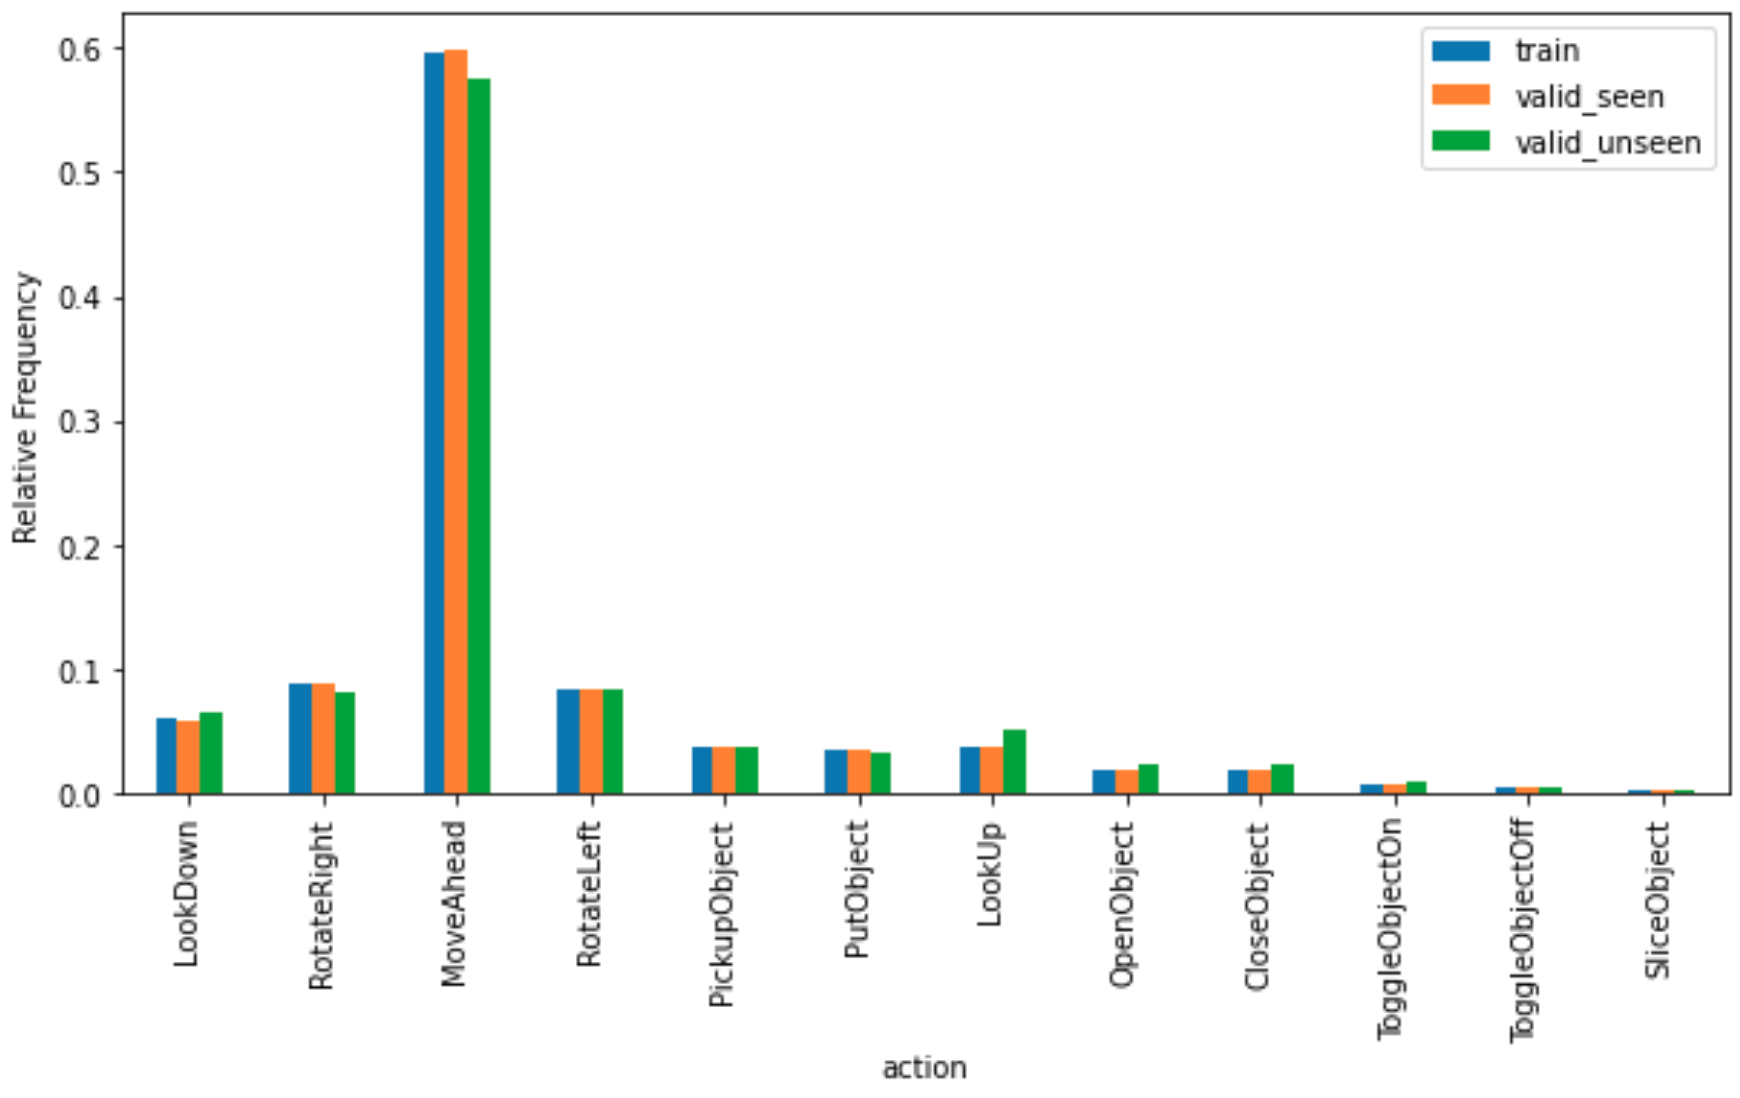
\includegraphics[scale=0.13]{figures/action_freq.png}
\caption{Relative frequency of each action type by split}
\label{fig:action-freq}
\end{figure}

Furthermore, Figure \ref{fig:action-freq} shows the frequency of the 12 different actions (5 navigation actions + 7 interaction actions). Note that all splits have fairly equal frequency for all actions. Also, note that 60\% of actions are ``move ahead'' actions which signifies the importance of a navigation module we may need in our model.

\subsubsection{Textual Analysis}
% important synonyms, and OOV 
For textual analysis, we first identified out of vocabulary (OOV) words in the training and validation set using a vocabulary of 685k words defined by spaCy. We found that less than 0.002\% of all words were OOV in any split, indicating the dataset is already quite clean. Most of the OOV words were just misspelled (eg: "stovve"), indicating that it would be important to preprocess text using a simple spell checker before using it for downstream tasks.

We also found the top few synonyms used to describe objects in the dataset. This was performed by comparing the similarity of word vectors of all objects in the dataset with all common nouns identified in all task descriptions. The complete results are in the Jupyter notebook, but a few results are shown in Table \ref{tab:synonynms}. This reveals that our model will need to be robust enough to recognize synonyms of different words in order to be successful. 

Furthermore, we analyzed how many objects present in the scene are directly referred to in the step-by-step instructions. The results are plotted in a histogram in Figure \ref{fig:object-vs-instruction}, which reveals that much less than 40\% of objects in the scene are actually referred to in the instructions. 

\begin{figure}[H]
\centering
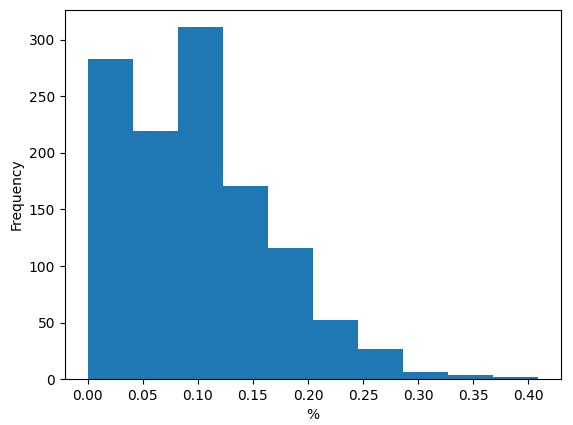
\includegraphics[scale=0.33]{figures/objects_vs_instructions.png}
\caption{Percentage of objects referred to in instructions compared to objects in the scene}
\label{fig:object-vs-instruction}
\end{figure}

\subsubsection{Visual Analysis}
% image sizes, which preprocessing techniques will help, visual quality
Due to compute constraints, most visual analysis was performed qualitatively by inspecting visual quality of different types of images. Figure \ref{fig:sample_ims} shows some sample RGB, depth and instance segmentation images. All images retrieved during simulation are of size 300 x 300.

% We also plan to apply the following three image augmentation methods to increase robustness of our models to unseen data: color jitter (for robustness in unseen lighting conditions), random perspective transformation (for robustness to object being viewed from different angles/perspectives), and random distortion (for general robustness to avoid over-fitting on specific objects seen in training). Note many other common augmentation methods like mirroring and cropping may not be applicable in our setting as they may unrealistically change/hide some objects in the scene.


\begin{table}[H]
\small
\begin{tabular}{@{}ll@{}}
\toprule
Object Name & Synonyms used in task descriptions  \\ \midrule
Coffee Machine & Espresso Machine, Beverage Machine \\
Chair & Couch Chair, Sofa Chair \\
CD   & DVD \\
Side Table & Corner Table \\
Butter Knife & Bread knife \\
Ottomon & Loveseat, Recliner \\
Fridge & Kitchen Fridge, Refrigerator \\
Poster & Wall Photo, Picture \\
Safe & Safety Box \\ 
Soap Bottle & Lotion Bottle
\end{tabular}

\caption{Synonyms (i.e. closest words in embedding space) used in task descriptions of some objects in the dataset}
\label{tab:synonynms}
\end{table}


\begin{figure*}
     \centering
     \begin{subfigure}[b]{0.32\textwidth}
         \centering
         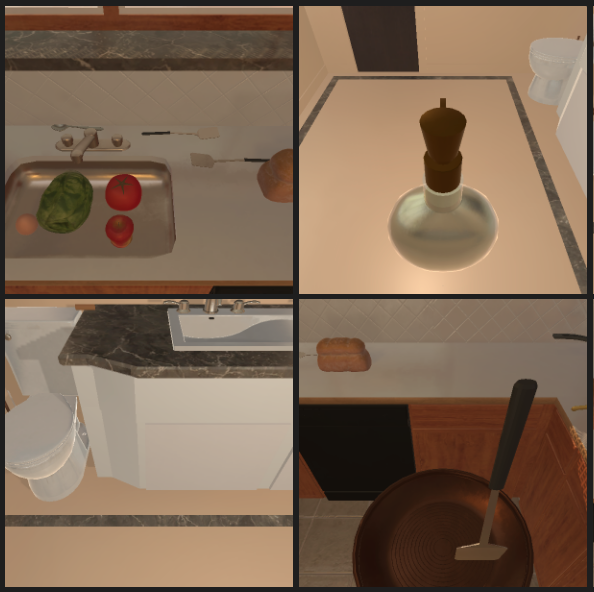
\includegraphics[width=\textwidth]{figures/rgb.png}
         \caption{}
     \end{subfigure}
     \hfill
     \begin{subfigure}[b]{0.32\textwidth}
         \centering
         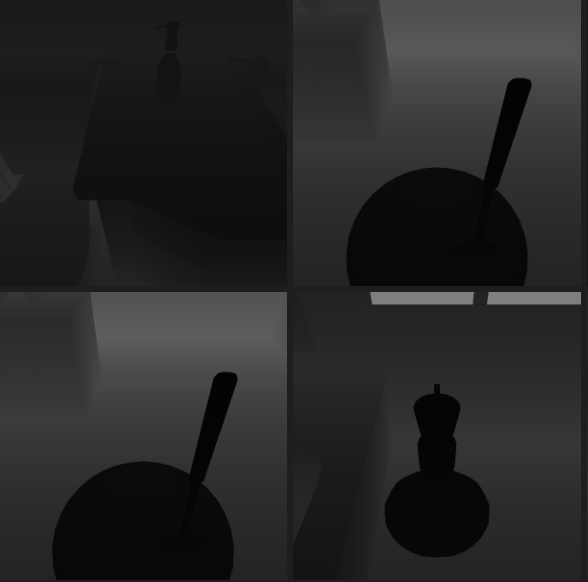
\includegraphics[width=\textwidth]{figures/depth.png}
         \caption{}
     \end{subfigure}
     \hfill
     \begin{subfigure}[b]{0.32\textwidth}
         \centering
         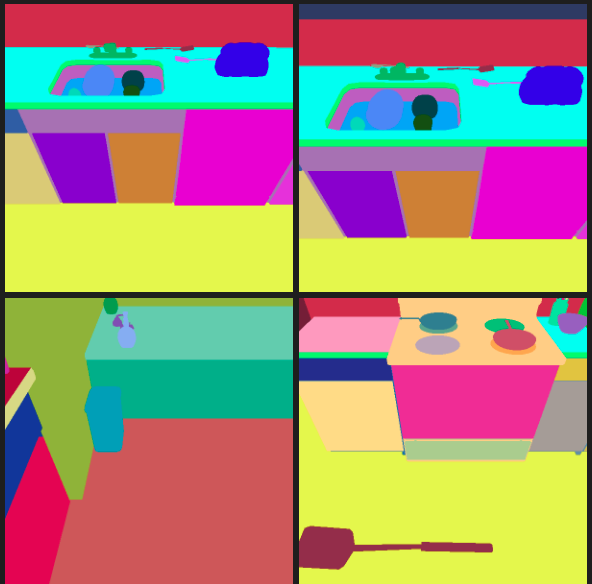
\includegraphics[width=\textwidth]{figures/seg.png}
         \caption{}
     \end{subfigure}
        \caption{Sample RGB, depth, and instance segmentation images retrieved from AI2Thor simulator}
        \label{fig:sample_ims}
\end{figure*}

\subsubsection{Other Qualitative Analysis}
% can a human do that?
In addition to the quantitative analysis, we also analyzed the solvability of the task. Our analysis in Figures \ref{fig:focus} and \ref{fig:dest} (in Appendix) shows that the unseen split of the validation set contains objects from the same classes as the training data, but could contain novel instances of those objects in novel environments. Since classes remain the same during training and testing times, the training data contains full information to solve the task, meaning a sufficiently intelligent agent should be able to solve the task, given training data.

\subsection{Metrics}
There are two primary metrics for evaluation. The first is ``task success'', which is a binary value indicating if the object positions and state changes correspond correctly to the goal-conditions of the task at the end of the action sequence. The second is ``goal-condition success'', which is the fraction of required goal-conditions that were completed at the end of the episode. Note that ``task success'' is true only if ``goal-condition success'' is 100\%. Additionally, there exists a path-weighted version of these two metrics that considers the length of the episode, penalizing longer action sequences. For example, in the path-weighted version, an agent would receive half the score for taking twice as long as an expert to complete the task.
% evaluation methods (Andrew)

\clearpage
\clearpage
\section{Models (2 pages)}

\subsection{Baselines}

% Baselines/Ablations:
    % uni-modal versions of current methods
    % what if we don't use LSTMs?
% Predefined metrics (defined by someone else):
    % All metrics from ALFRED 3.2 section
    % Sub-goal evaluation (as explained in ALFRED)
        % check how this is implemented
        % does this use info from expert trajectories to measure completion of each sub-goal? If yes, which expert trajectory does it use because there are 3?
        % Since most models use some form of LSTM, how can we randomly spawn agents at any place and expect same performance because the LSTM hidden state would not have had a chance to get updated correctly?
% Intrinsic Metrics (defined by us):
    % Navigation: percent of times we reach within distance x of the first object that should be interacted with
        % orientation of agent - is it facing the right object?
    % Interaction Action Prediction: percent of times you predict the right interaction action when you were near the right object
    % Instance Segmentation: given that we are in the right location and we predict the right action, do you get the correct segmentation mask? 
        % group by object class, interaction mask size
    % Length Conditioned Success: the average first n sub-goal achieved without using expert resetting
    % Sub-goal evaluation (as explained in ALFRED) grouped by goal completion index divided by total sub goals
        % plot using x-axis = normalized sub-goal index, y-axis = sub-goal evaluation
        % should also try grouping by task type
        % grouped by action type
    % Note: all metrics can be grouped by task type, seen/unseen, environment type, expert trajectory length (short, medium, long)
    % we can use attention scores to see if the right object is being focused on
        % the exact details of how this will happen are not clear, but can be clarified once the approach is ready
% Empty results table
    % includes all metrics defined above
    % find out which models use depth and image segmentation masks, note this in the results
    % find out if code is available
    % models of interest:
        % moVILAN
        % MOCA
        % ALFRED baseline
        % Modularity improves out of domain generalization
        % Ours
        

\subsubsection{Baselines and Other Methods}
\label{sssec:baselines}
We plan to use the following baselines/other SOTA methods for comparison purposes. In the following, we only cite previous approaches (without explanation) as they have been described in detail in Section \ref{sec:rel-work}, but describe our proposed baseline approach in detail. 
\begin{itemize}
\item \textbf{Seq-2-Seq (CNN-LSTM)} \cite{shridhar2020alfred} % a CNN encodes the visual input while a bi-directional LSTM encodes the language input and a decoder LSTM infers low-level actions while attending over encoded language.

\item \textbf{Seq-2-Seq PM} \cite{shridhar2020alfred} % Seq-2-Seq with progress monitors uses two additional losses that help the agent know which sub-goals have been completed (coarse progress estimation) and predict which timestep of the expert demonstration it is currently on.

\item \textbf{Modular Seq-2-Seq} \cite{corona2020modularity}

\item \textbf{MOCA} \cite{singh2020moca} 

\item \textbf{Seq-2-Seq RL (proposed):}  Since we may likely use a reinforcement learning (RL) based approach, we plan to use the same Seq-2-Seq PM architecture and train it using a standard RL algorithm like PPO to get a baseline \cite{schulman2017proximal}. While it is hard to determine the exact reward function without any experimentation, some possible reward functions to try could be a combination of task completion, an intrinsic reward like curiosity \cite{burda2018large}, and possibly an imitation learning (IL) reward as proposed by \newcite{reddy2019sqil}. We could also add a reward that forces the agent to go towards objects in the order of the expert and interact with them in similar ways. Since the task is long and the reward could be sparse, we also intend to warm start the policy using IL as proposed in many previous approaches \cite{rajeswaran2017learning,wang2019reinforced}.
\end{itemize}

% \subsubsection{Current Results}
% See Table \ref{tab:results} for baseline and current results on ALFRED.

\subsubsection{Proposed Ablations}
\newcite{shridhar2020alfred} perform an input ablation study for their baseline Seq2Seq approach. They individually remove four inputs from the model: language, vision, the step-by-step instructions, and the goal statement, and evaluate the model's performance in each case. MOCA \cite{singh2020moca} performs the same ablation study as well, and we also plan to conduct this study on our model.

In addition to ablating the inputs to our model, we also plan to perform an ablation study over the training method. While our modeling plans have not been finalized, we currently are interested in exploring an RL-based approach. To empirically verify if RL performs better than IL, we plan to train two variants of our model: one trained using RL, and the other trained using simple IL like other approaches.

\subsubsection{Metrics}
We plan to use the following existing metrics to evaluate our approach.
\begin{enumerate}
    \item \textbf{Task success (TS)}: TS is simply a binary value indicating whether the overall task has been completed. The task is considered complete if the final states and positions of objects of interest in the trajectory align with expected states.
    \item \textbf{Goal-conditioned success (GCS)}: This is the ratio of goal-conditions completed at the end of the episode to the total number of goal-conditions required for task success. By definition, GCS is more granular than TS.
    \item \textbf{Path Weighted Metrics}: We can also compute the path weighted versions of TS and GCS. So, if the model takes twice as many actions has the expert, the original TS and GCS scores would decrease by half.
\end{enumerate}

In addition to computing the above metrics on the entire ALFRED task, we will also compute them at the sub-goal level by moving the agent through the expert trajectory before the sub-goal, and then letting it complete the sub-goal. This was also performed by \newcite{shridhar2020alfred}.

Moreover, to better identify performance bottlenecks in ours and other approaches, we propose the following other metrics:

\begin{enumerate}
    \item \textbf{Navigation Performance (NP)}: NP is the percentage of times the agent can come within a certain distance of the first object (and also face the correct object) it has to interact with for each sub goal. Note that we are only concerned with the first object of interaction because subsequent actions may involve interaction actions, making it difficult to reliably attribute credit of future success/failure to navigation alone. A high percentage would indicate that the agent is successfully able to at least navigate to the object of interest, indicating navigation may not necessarily be a performance bottleneck.
    \item \textbf{Interaction Mask Prediction Performance (IMPP)}: Of all the times the agent predicts the correct interaction action near the correct object, IMPP is defined as the intersection over union score of the predicted instance segmentation mask with respect to the ground truth mask. Since IMPP is conditioned on the interaction action being correct, IMPP only measures the performance of the component that predicts the interaction mask. We also plan to measure IMPP grouped by object class to understand whether certain objects are more difficult to identify.
    \item \textbf{Interaction Action Prediction Performance (IAPP)}: IAPP is the percent of times the model predicts the right interaction action when it has identified the instance segmentation mask of the correct object.
    \item \textbf{Length-conditioned Success (LCS)}: LCS is the first $n$ sub-goals successfully completed continuously. A low LCS indicates that the policy is struggling to complete tasks that have higher number of instructions.
\end{enumerate}

Note that a recurring theme in most proposed metrics is to measure performance over each aspect needed to solve the task in as much isolation as possible. For example, we try to measure navigation and interaction performance separately by using NP, IMPP, and IAPP as proposed above.

In addition to the above base metrics, we also plan to use several of their more fine-grained variations to better understand model performance. Specifically, we plan to group all metric calculations by task type, environment type (i.e. room, kitchen, bathroom), expert trajectory length (i.e short, medium, high) to understand models at a more fine-grained level.

\subsubsection{Empty results table}
As mentioned in \ref{sssec:baselines}, we intend to compare our approach to five other approaches. Since \newcite{corona2020modularity} do not report overall task success rate, we only use their goal-condition success metric for comparison. Note that the baseline approach is the highest-performing variant of their Seq2Seq model, specifically the model with both progress and sub-goal progress monitoring enabled. To the best of our knowledge, the methods we compare to are currently the only approaches that attempt the official ALFRED task as defined by \newcite{shridhar2020alfred} and are eligible for the ALFRED leaderboard.  In particular, \newcite{Storks2021AreWT} only evaluate on the \textbf{Stack \& Place} task, and \newcite{Saha2021AMV} make use of depth map information from the simulator and use a different train/test split than the official benchmark, thus making both approaches not easily comparable. We report our overall results in Table \ref{tab:results}. Additionally, we report results for our proposed intrinsic metrics on the validation set and compare to the baseline model in Table \ref{tab:intrinsic}.




\begin{table*}[]
\centering
\resizebox{\textwidth}{!}
{\begin{tabular}{@{}lllllllll@{}}
\toprule
                         & \multicolumn{4}{c}{\textbf{Validation}}                                                                             & \multicolumn{4}{c}{\textbf{Test}}                                                                                   \\
                         & \multicolumn{2}{c}{\textit{Seen}}                        & \multicolumn{2}{c}{\textit{Unseen}}                      & \multicolumn{2}{c}{\textit{Seen}}                        & \multicolumn{2}{c}{\textit{Unseen}}                      \\
Model                    & \multicolumn{1}{c}{Task} & \multicolumn{1}{c}{Goal-Cond} & \multicolumn{1}{c}{Task} & \multicolumn{1}{c}{Goal-Cond} & \multicolumn{1}{c}{Task} & \multicolumn{1}{c}{Goal-Cond} & \multicolumn{1}{c}{Task} & \multicolumn{1}{c}{Goal-Cond} \\ \midrule
\textbf{Baselines}       &                          &                               &                          &                               &                          &                               &                          &                               \\
Seq2Seq \cite{shridhar2020alfred}                  & 2.4 (1.1)                & 9.4 (5.7)                     & 0.1 (0.0)                & 6.8 (4.7)                     & 2.1 (1.0)                & 7.4 (4.7)                     & 0.5 (0.2)                & 7.1 (4.5)                     \\
+ PM Progress-Only       & 2.1 (1.1)                & 8.7 (5.6)                     & 0.0 (0.0)                & 6.9 (5.0)                     & 3.0 (1.7)                & 8.0 (5.5)                     & 0.3 (0.1)                & 7.3 (4.5)                     \\
+ PM Subgoal-Only        & 2.1 (1.2)                & 9.6 (5.5)                     & 0.0 (0.0)                & 6.6 (4.6)                     & 3.8 (1.7)                & 8.9 (5.6)                     & 0.5 (0.2)                & 7.1 (4.5)                     \\
+ PM Both                & 3.70 (2.10)              & 10.00 (7.00)                  & 0.00 (0.00)              & 6.90 (5.10)                   & 3.98 (2.02)              & 9.42 (6.27)                   & 0.39 (0.80)              & 7.03 (4.26)                   \\
+ RL (proposed baseline)                &    &          &     &          &     &                   &     &                         \\ \midrule
Modular \cite{corona2020modularity}          & \multicolumn{1}{c}{-}    & \multicolumn{1}{c}{-}         & \multicolumn{1}{c}{-}    & \multicolumn{1}{c}{-}         & \multicolumn{1}{c}{-}    & 8.80 (6.30)                   & \multicolumn{1}{c}{-}    & 7.20 (5.70)                   \\
MOCA \cite{singh2020moca}                     & 19.15 (13.60)            & 28.50 (22.30)                 & 3.78 (2.00)              & 13.40 (8.30)                  & 22.05 (15.10)            & 28.29 (22.05)                 & 5.30 (2.72)              & 14.28 (9.99)                  \\
\textbf{Ours}            &                          &                               &                          &                               &                          &                               &                          &                               \\ \midrule
Human                    & \multicolumn{1}{c}{-}    & \multicolumn{1}{c}{-}         & \multicolumn{1}{c}{-}    & \multicolumn{1}{c}{-}         & \multicolumn{1}{c}{-}    & \multicolumn{1}{c}{-}         & 91.00 (85.80)            & 94.50 (87.60)                 \\ \midrule
\textbf{Ablations} &                          &                               &                          &                               &                          &                               &                          &                               \\
No Language              &                          &                               &                          &                               &                          &                               &                          &                               \\
No Vision                &                          &                               &                          &                               &                          &                               &                          &                               \\
Goal-Only                &                          &                               &                          &                               &                          &                               &                          &                               \\
Instructions-Only        &                          &                               &                          &                               &                          &                               &                          &                               \\
Trained using IL only       &                          &                               &                          &                               &                          &                               &                          &                               \\\bottomrule
\end{tabular}}
\caption{\textbf{Task and Goal-Condition Success Rate.} Corresponding path-weighted metrics are given in parentheses.}
\label{tab:results}
\end{table*}


\begin{table*}[]
\begin{tabular}{@{}lllllllll@{}}
\toprule
                         & \multicolumn{4}{c}{\textit{Seen}} & \multicolumn{4}{c}{\textit{Unseen}} \\ \midrule
Model                    & NP    & IMPP    & IAPP    & LCS   & NP     & IMPP    & IAPP    & LCS    \\ \midrule
\textbf{Baselines}       &       &         &         &       &        &         &         &        \\
Seq2Seq                  &       &         &         &       &        &         &         &        \\
+ PM Progress-Only       &       &         &         &       &        &         &         &        \\
+ PM SubGoal-Only        &       &         &         &       &        &         &         &        \\
+ PM Both                &       &         &         &       &        &         &         &        \\
+ RL (proposed baseline)                &       &         &         &       &        &         &         &        \\ \midrule
\textbf{Ours}            &       &         &         &       &        &         &         &        \\ \midrule
\textbf{Ablations} &       &         &         &       &        &         &         &        \\
No Language              &       &         &         &       &        &         &         &        \\
No Vision                &       &         &         &       &        &         &         &        \\
Goal-Only                &       &         &         &       &        &         &         &        \\
Instructions-Only        &       &         &         &       &        &         &         &        \\
Trained using IL only        &       &         &         &       &        &         &         &        \\
\bottomrule
\end{tabular}
\caption{\textbf{Intrinsic Metrics - Validation.}}
\label{tab:intrinsic}
\end{table*}


\subsection{Proposed Approach}

\clearpage

\section{Results (1 page)}
The columns above are just examples that should be expanded to include all metrics and baselines.

\clearpage
\section{Analysis (2 pages)}
This section should include at least two to three plots
\subsection{Ablations and Their Implications}

\subsection{Qualitative Analysis and Examples}
This section should likely contain a table of examples demonstrating how the current approach succeeds/fails.

% Please use 
\bibliographystyle{acl_natbib}
\bibliography{references}

%\appendix
\clearpage
\section{Appendix}

\begin{figure*}
    \centering
    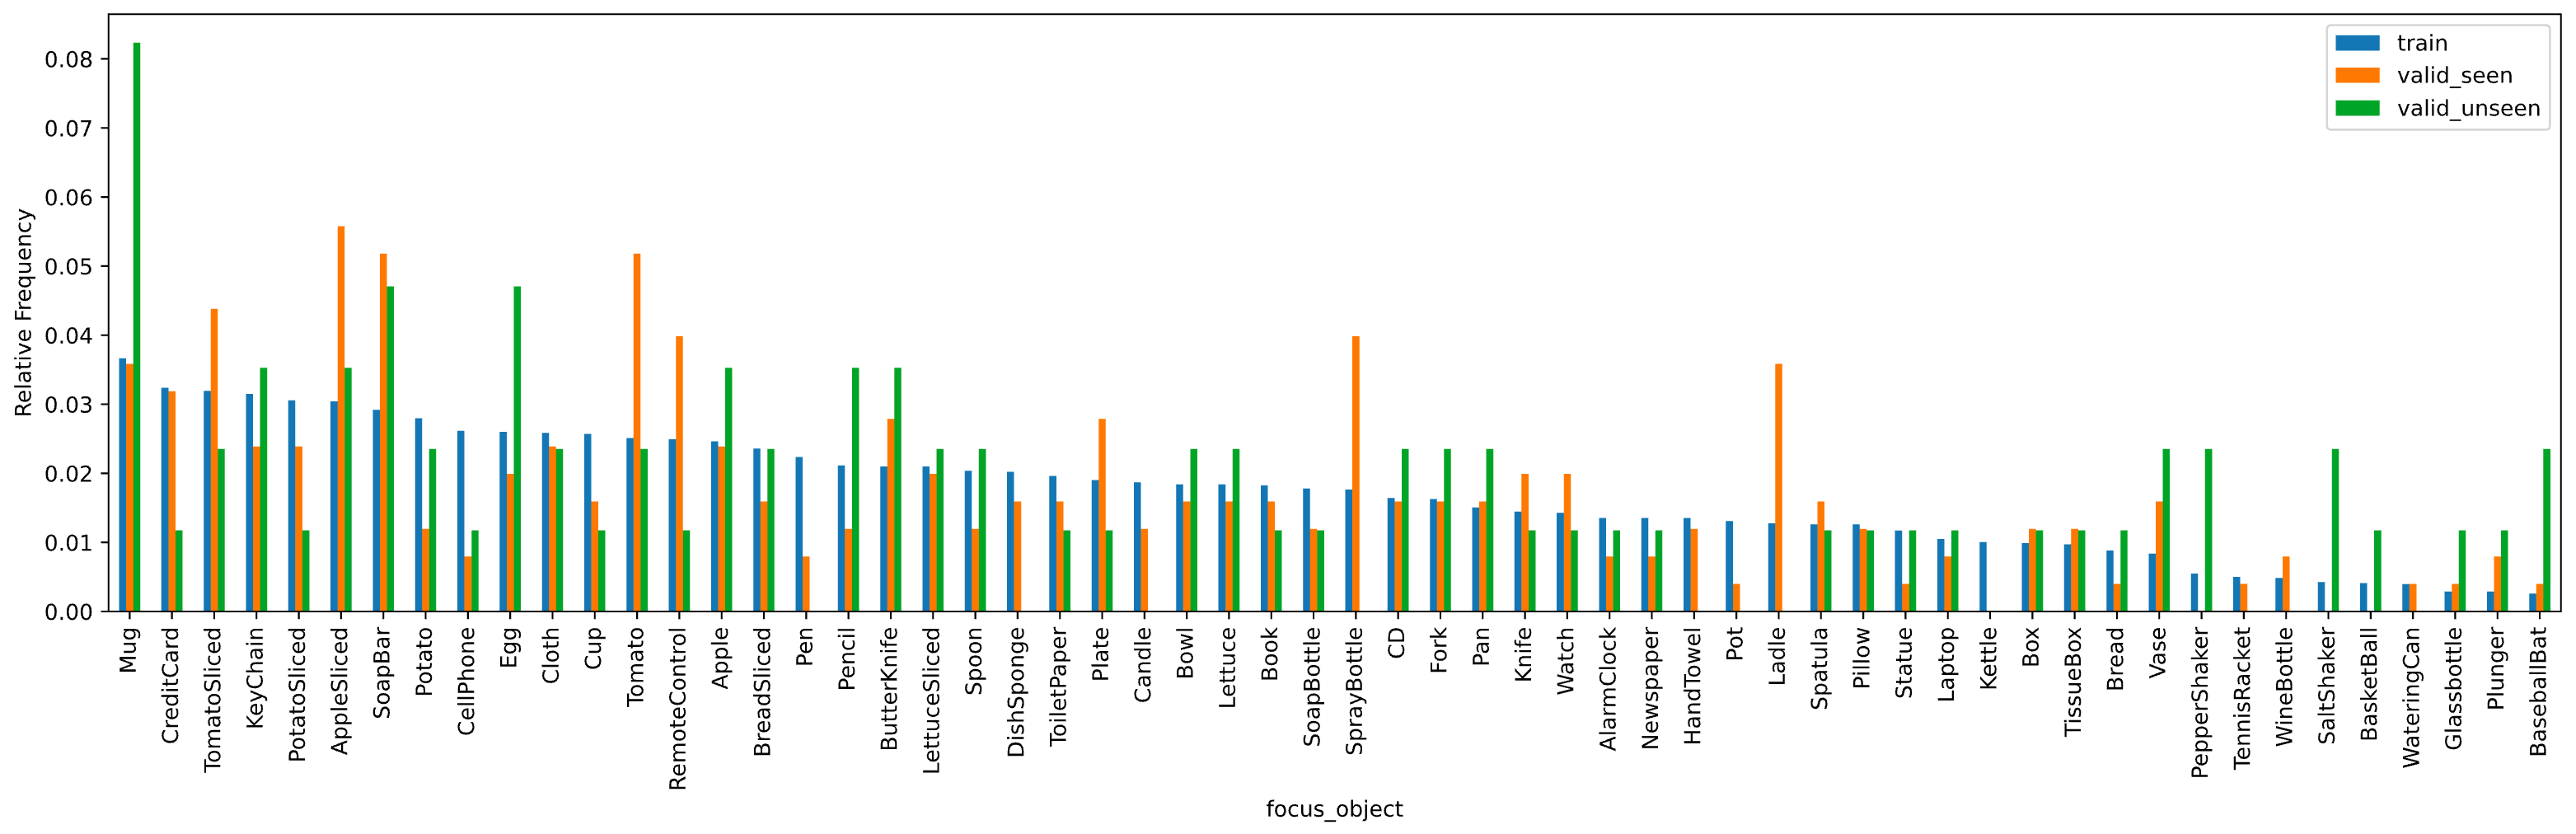
\includegraphics[scale=0.3]{figures/focus_obj_freqs.png}
    \caption{Relative frequency of focus objects used in different splits}
    \label{fig:focus}
\end{figure*}

\begin{figure*}
    \centering
    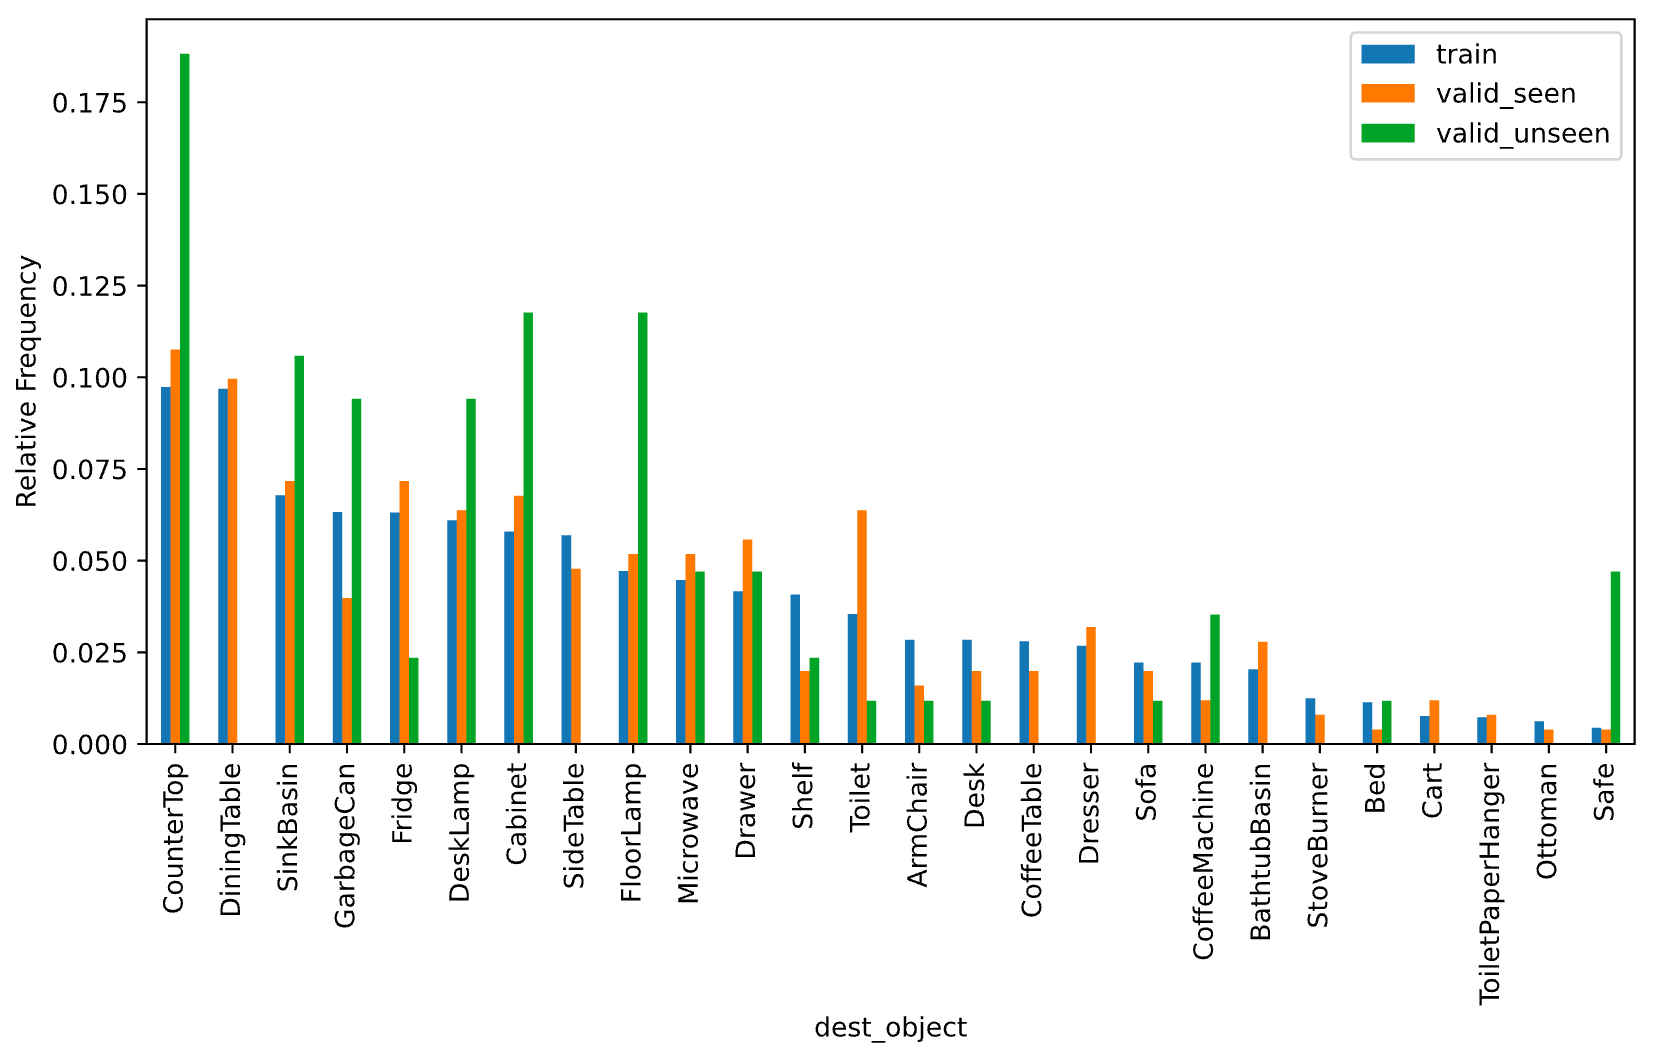
\includegraphics[scale=0.5]{figures/dest_obj_freqs.png}
    \caption{Relative frequency of destination objects used in different splits}
    \label{fig:dest}
\end{figure*}


\subsection{Data Analysis Plots}

Description of fields in Table \ref{fig:action-freq}:
\begin{enumerate}
    \item Steps per directive: number of steps in each language directive
    \item Tokens per step: number of words in each directive step
    \item Task description tokens: number of words in directive task description
    \item Images: number of images per demonstration
    \item Actions: number of actions per demonstration
    \item Images per action: number of images divided by number of actions per demonstration
    \item Actions per step: number of actions divided by number of directive steps per demonstration
    \item Nav-interact ratio: number of navigation actions divided by number of interaction actions per demonstration
    \item Total objects: number of total objects in a scene per demonstration
    \item Mask coverage: proportion of the image that is covered by the interaction mask per demonstration
    \item Step-object coverage: proportion of interaction actions whose object of interest is mentioned in the step-by-step instructions, averaged over all interaction actions and language directives in the demonstration
\end{enumerate}

In Figure \ref{fig:task-type}, we see that ALFRED contains a roughly equal number of demonstrations for each type of task, and for the most part, a roughly equal proportion for each split. The validation data, especially the unseen portion, does have relatively less ``Pick Two \& Place'' tasks than the training data. Additionally, the unseen portion has a significantly higher proportion of ``Examine in Light'' tasks than the other splits.

\begin{figure}[H]
\centering
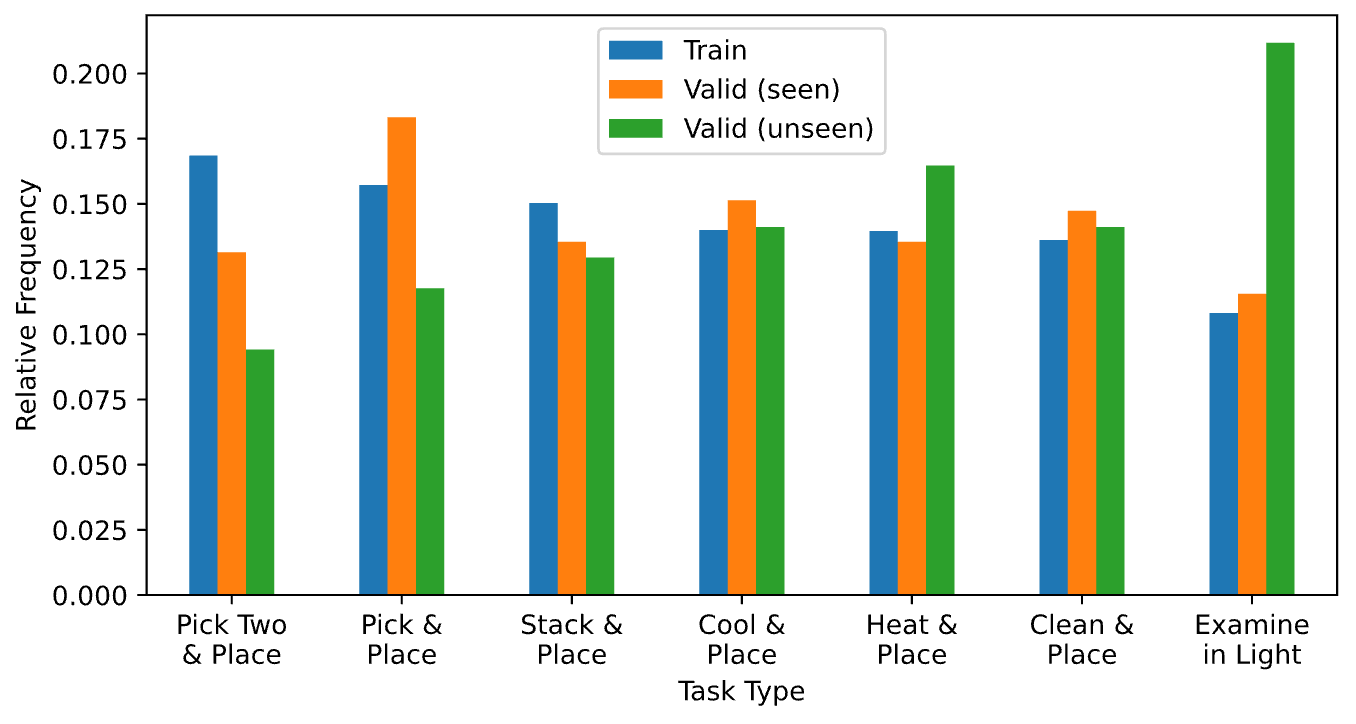
\includegraphics[scale=0.33]{figures/task_type_freqs.png}
\caption{Relative frequency of each task type by split}
\label{fig:task-type}
\end{figure}

\end{document}
